\documentclass[12pt,a4paper,notitlepage,twoside,headsepline]{scrartcl}
\usepackage{pstool}
\usepackage{booktabs}
\usepackage[T1]{fontenc}
%\usepackage[latin1]{inputenc}
\usepackage{amsmath, amssymb, amsthm}
\usepackage{scrpage2}
\usepackage{lmodern}
\usepackage{microtype}
\usepackage[english]{babel}
\usepackage{mathtools}
\usepackage{caption}
\usepackage{subcaption}
% \usepackage{hyperref}
%%%%%%%%%%%%%%%%%%%%%%%%%%%%%%%%%%%%%%%%%%%%%%%%%%%%%%%%%%%%%%%%%%%%%%%%%%%%%%%
\def\ve#1{{\mathchoice{\mbox{\boldmath$\displaystyle #1$}}%
              {\mbox{\boldmath$\textstyle #1$}}%
              {\mbox{\boldmath$\scriptstyle #1$}}%
              {\mbox{\boldmath$\scriptscriptstyle #1$}}}}

%%%% Laengen %%%%%%%%%%%%%%%%%%%%%%%%%%%%%%%%%%%%%%%%%%%%%%%%%%%%%%%%%%%%%%%%%%
\unitlength1cm
\setcounter{secnumdepth}{5}
\setcounter{tocdepth}{5}
\textwidth=17cm
\textheight=23.5cm
\hoffset=-20mm
%\voffset=-10mm
\parindent0cm
\parskip.5em plus.1em minus .2em
\headheight6mm
\headsep8mm
\footskip22mm
\oddsidemargin16.0mm
\evensidemargin11.5mm
\renewcommand{\baselinestretch}{1.1}

%%%%%%%%%%%%%%%%%%%%%%%%%%%%%%%%%%%%%%%%%%%%%%%%%%%%%%%%%%%%%%%%%%%%%%%%%%%%%%%
% commands
\newcommand{\R}{\mathbb{R}}
\newcommand{\Z}{\mathbb{Z}}
\newcommand{\N}{\mathbb{N}}
\newcommand{\C}{\mathbb{C}}
\newcommand{\Q}{\mathbb{Q}}
\newcommand{\F}{\mathbb{F}}

%%%%%%%%%%%%%%%%%%%%%%%%%%%%%%%%%%%%%%%%%%%%%%%%%%%%%%%%%%%%%%%%%%%%%%%%%%%%%%%


%%%%%%%%%%%%%%%%%%%%%%%%%%%%%%%%%%%%%%%%%%%
% Pagestyle
\pagestyle{headings}
\clearscrheadfoot
\ihead{Interference Alignment for SC-FDMA Systems with Widely Linear Filtering}	% Add the title of the document here.
\ohead{\pagemark}
%%%%%%%%%%%%%%%%%%%%%%%%%%%%%%%%%%%%%%%%%%%
\EndPreamble % required by \pstool

% Begin of document
\begin{document}

\begin{titlepage}
\title{
\begin{center}
    \textbf {Research Internship}  \\[0.5cm]  
    \textbf{\Large\ Interference Alignment for SC-FDMA Systems with Widely Linear Filtering}  \\ [0.3cm]
    \textbf{\Large Mohamed Soliman} \\[0.3cm]    
    \textbf{\small Supervisor}\\[0.3cm]
    \textbf{\small Dipl.-Ing. Uyen Ly Dang}\\[0.1cm]
	\textbf{\small Prof. Dr.- Ing Wolfgang Gerstacker}\\[0.1cm]				
\end{center}
}
%\author{Mohamed Soliman}
\date{December 22, 2017}
\end{titlepage}

%%%%%%%%%%%%%%%%%%%%%%%%%%%%%%%%%%%%%%%%%%%%
\maketitle

\section*{Abstract}
In expectation of growing interference level in cellular systems in the near future, elaborate interference management techniques are necessary in addition to the traditional interference avoidance approaches employed so far. Here, we investigate widely linear filtering at the transmitter and the receiver side to overcome the issue associated with limited number of signaling dimensions. We consider transmit beamforming for single carrier frequency division multiple access (SC-FDMA) transmission over frequency selective multiple-input multiple-output (MIMO) channels, assuming that the data symbols are mapped into points of fixed signal constellations, a transceiver structure employing widely linear (WL) filters, rather than linear ones, is proposed in order to exploit the statistical redundancy of some constellations, i.e., the correlation between the signals and their conjugate version. WL filters linearly and independently process both the in-phase and the quadrature components of the input signals and, with a limited increase in the computational complexity, allows one to improve the system performances.

%%%%%%%%%%%%%%%%%%%%%%%%%%%%%%%%%%%%%%%%%%%%
\section{Introduction}

%We begin with the introduction by using the 
%\verb|\section{Introduction}| command.


One of the main problems for wireless multimedia applications is the demand for higher data rate which leads to a wider transmission bandwidth. With the use of wider bandwidth comes through the issue of frequency selectivity thus the channel becomes severe alongside the inter-symbol interference (ISI). One way to solve frequency selective fading is using multi-carrier techniques which subdivide the channel into smaller sub-bands, or sub-carriers. Orthogonal frequency division multiplexing (OFDM) is a multicarrier modulation technique which uses orthogonal sub-carriers to convey information. To simplify the equalization process, each sub-carrier is seen as flat fading channel since the bandwidth of a sub-carrier is deigned to be smaller than the coherence bandwidth. On the other hand, in the time domain, OFDM resolves the problem of ISI by splitting a high-rate data stream into lower-rate data stream which is transmitted in parallel. However, OFDM has its disadvantages: high peak to average power ratio (PAPR), high sensitivity to frequency offset and the spectral nulls in the channel.


%%%%%%%%%%%%%%%%%%%%%%%%%%%%%%%%%%%%%%%%%%%%
\section{SC-FDMA}

\begin{figure}[!ht]
\begin{center}
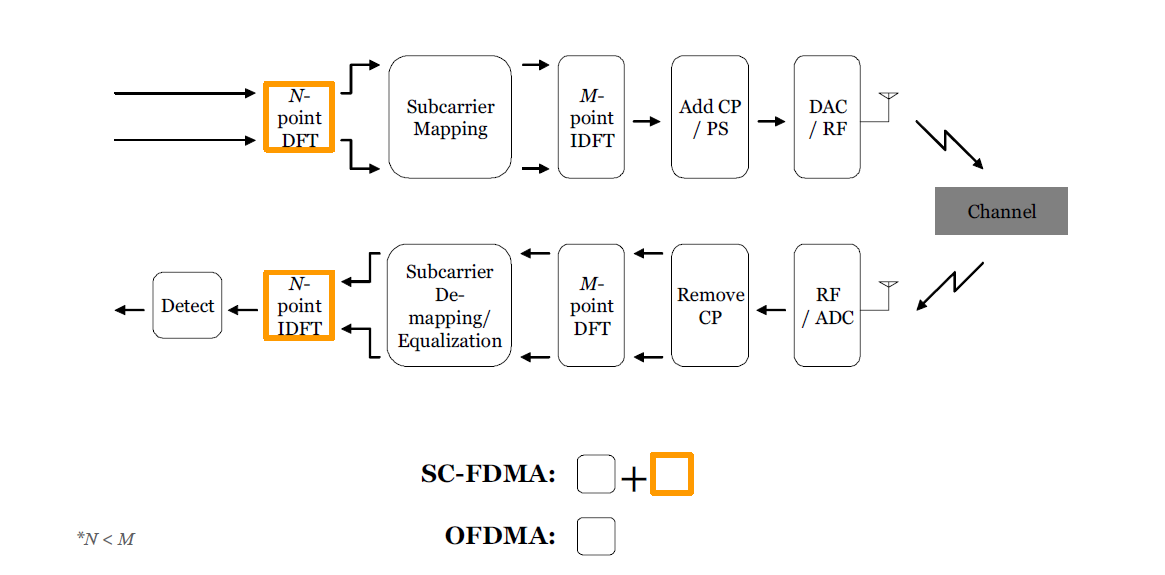
\includegraphics[width=0.7\textwidth]{figures/fig1}
\end{center}
\caption{Block diagram of an SC-FDMA transceiver.} %\cite{Example09}.
\label{fig:example}
\end{figure}


Single carrier frequency division multiple access (SC-FDMA) system which is a newly developed multiple access scheme adopted in the uplink of 3GPP Long Term Evolution (LTE),  has drawn great attention as an attractive alternative to OFDMA, especially in the uplink communications where lower PAPR greatly benefits the mobile terminal in terms of transmit power efficiency. Figure [] shows a block diagram of an SC-FDMA system. Basically, SC-FDMA system follows the same principle as OFDMA of using inverse discrete Fourier transform (IDFT) to transmit data symbols and discrete Fourier transform (DFT) to receive data symbols, with additional form of precoding by using DFT at transmitter and IDFT at receiver. The overall transmit signal is a single carrier signal, PAPR is inherently low compared to the case of OFDMA which produces a multi-carrier signal. 

The transmitter first groups the modulation symbols into blocks that contains N symbols. Then it performs the N-point DFT to produce frequency domain representation of the input symbols. After that, it maps each of the N symbols to M orthogonal sub-carriers that can be transmitted. Usually, M is greater than N (M>N). And finally, as in OFDMA system, the M-point IDFT transform the subcarrier amplitudes to the complex time domain signal. After the transmitter finishes with these blocks, it inserts a set of symbols as it called cyclic prefix (CP) in order to provide a guard interval that used to prevent inter-block interference (IBI) due to multipath propagation. Essentially, CP is a copy of the last part of the block, which is added to the start of the block as it acts like a guard interval between successive blocks. Usually, the length of CP is greater than the maximum delay spread of the channel or roughly the length of the channel impulse response, which will solve the problem of IBI. Also, by using CP as a copy of the last part of the block, it converts a discrete time linear convolution into a discrete time circular convolution. After the transmitter finishes with adding CP, it performs pulse shaping as a linear filtering operation in order to reduce the out of band signal energy.

\begin{figure}[!ht]
\begin{center}
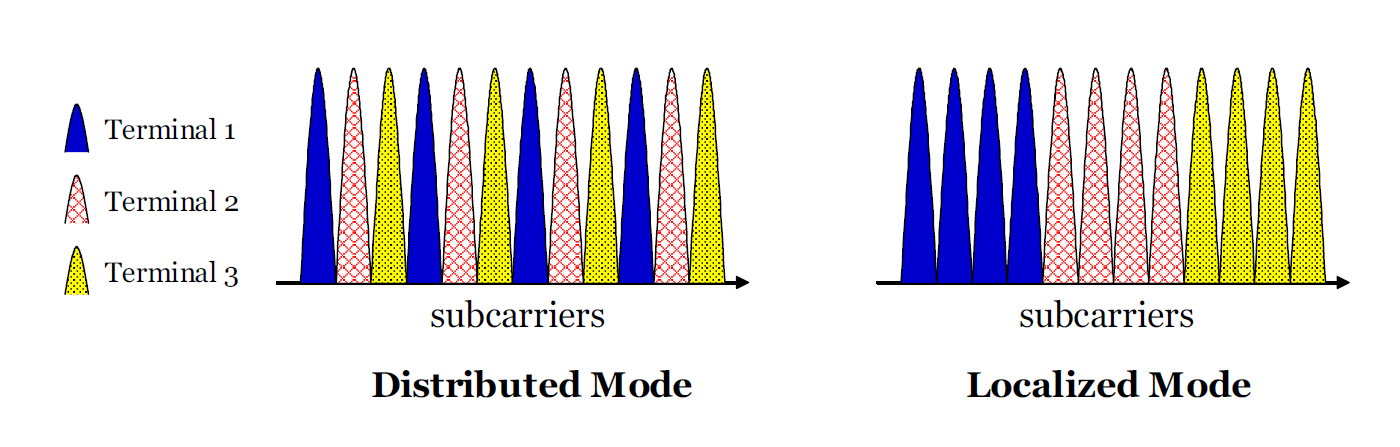
\includegraphics[width=0.7\textwidth]{figures/fig2}
\end{center}
\caption{Sub-carrier mapping within distribution mode and localized mode.} %\cite{Example09}.
\label{fig:example}
\end{figure}

Basically, there are two modes for sub-carrier mapping, distributed and localized.  In distributed sub-carrier mapping mode, DFT outputs of the input data are allocated over the entire bandwidth with zeros occupying the unused sub-carriers. For the localized sub-carrier mapping mode, consecutive sub-carriers are occupied by the DFT outputs of the input data, as shown in figure 2.


\begin{figure}[!ht]
\begin{center}
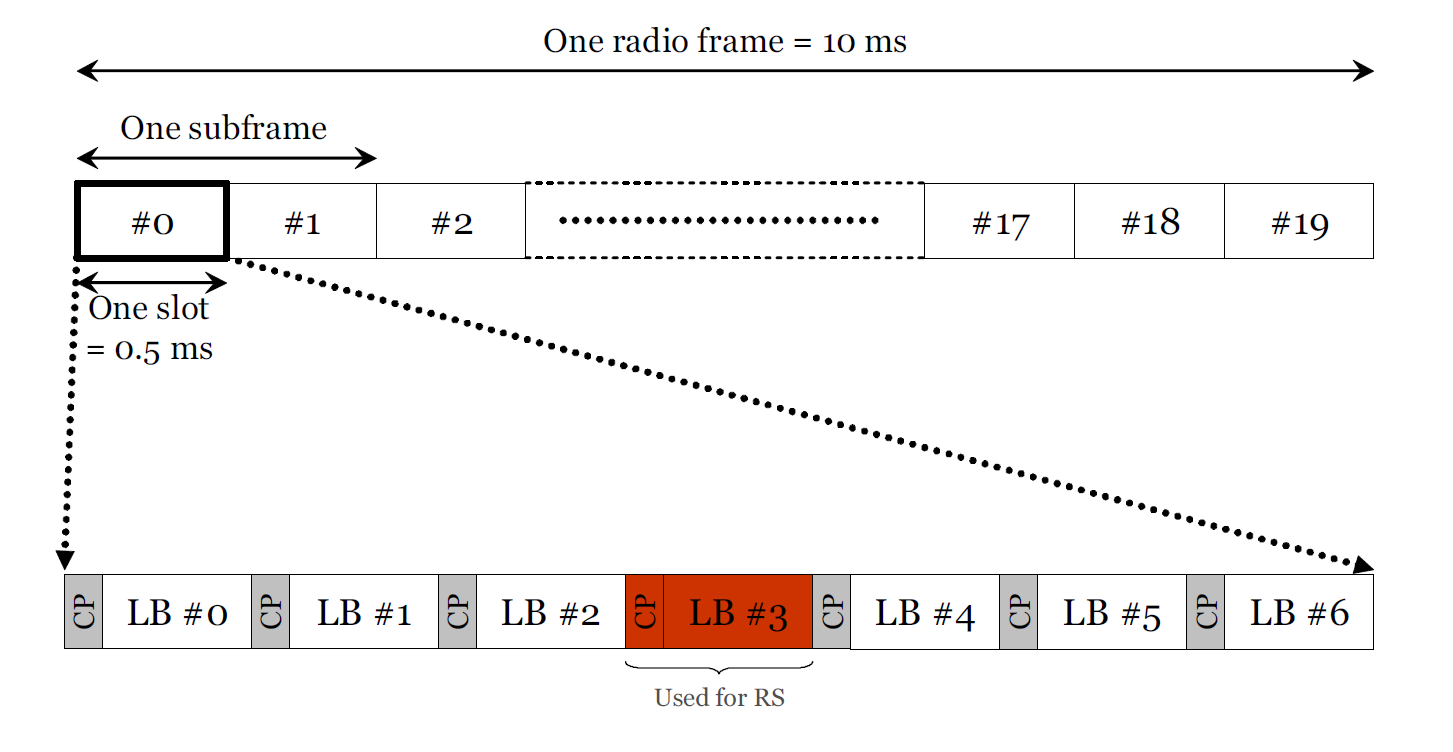
\includegraphics[width=0.7\textwidth]{figures/fig3}
\end{center}
\caption{Frame/slot structure in 3GPP LTE SC-FDMA uplink} 
\label{fig:example}
\end{figure}


Figure 3 illustrates the frame/slot structure of the time domain, one radio frame has duration of 10 ms and it consists of 20 slots. Also, two slots considered as a sub-frame. One slot consists of 7 long blocks (LB) with CP. The middle LB is used for reference signal (RS), or pilot signal. In the frequency domain, a resource block (RB) spans 12 sub-carriers over one slot duration of 0.5 ms and one sub-carrier has bandwidth of 15 kHz.


%%%%%%%%%%%%%%%%%%%%%%%%%%%%%%%%%%%%%%%%%%%%
\section{Interference alignment}

The SC-FDMA scheme is constrained in its user capacity by the length of the M-point DFT and N-point IDFT. Therefore, if every user has M data carrying sub-carriers and there is an available N-sub-carrier mapping space, we can only accommodate

\begin{equation}
	T = N/M
\end{equation}


Users in the system if we aim for a completely disjoint sub-carrier distribution, i.e., not allowing for any interference between the users. So, to increase the user-capacity for such a system without changing the available frequency resources (M and N), we have to find a way to allow users to use the same sub-carrier space and manage the interference seen at each receive terminal. To overcome the interference problem, interference alignment is the concept that will be used in this case. Interference alignment is the interference management strategy which exploits the availability of multiple signaling dimensions provided by multiple time slots, frequency blocks, or antennas. 

\subsection{Strictly linear filter}

Strictly linear filtering is a transmission scheme where all transmitters linearly encode their signals over multiple dimensions which maximizes the number of non-interfering symbols. These symbols can be simultaneously transmitted over an interfering channel so that at each receiver the interfering signals will be align at low dimension subspace. Basically, interference alignment allows users to use precoding at their transmissions jointly such that each two interference signals are fully contained in one dimensional subspace. So that, the alignment leaves one dimension where users can decode their received signal with interference-free by projecting the received signal into the subspace orthogonal to the interference subspace.


\subsection{Widely linear filter}

Widely linear filtering generalizes linear filtering by linearly processing the in-phase and quadrature components of the input signals separately, without requiring a significant increase in the computational complexity which achieve significant performance improvement by exploiting the correlation between signals and their conjugate version. The imaginary and the real part of the filter input are processed separately and subsequently combined linearly. When additionally applying real-valued transmit symbols, a WL system model results which has doubled dimensions. This translates into more degrees of freedom for the filter design.

%%%%%%%%%%%%%%%%%%%%%%%%%%%%%%%%%%%%%%%%%%%%%%%%%%%%%%%%%%%%%%%%%%%%%%%%%%%%%%%
\section{System Model}

In our system model, we consider an SC-FDMA scheme with a K-user MIMO interference network, where each transmitter and receiver is equipped with $Nt$ transmit antennas and $Nr$ receive antennas. We introduce interference alignment solution by the additional of precoding. We discuss about two main cases with different types of filters used in precoding, strictly linear filter and widely linear filter. 

\subsection{Strictly linear filter}

\begin{figure}[!ht]
\begin{center}
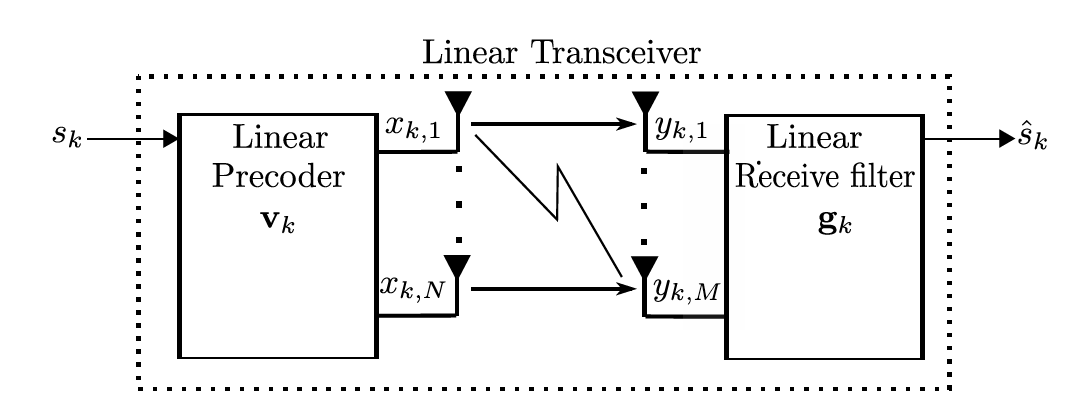
\includegraphics[width=0.7\textwidth]{figures/sl_system_model.png}
\end{center}
\caption{Block diagram of Linear Transceiver} 
\label{fig:example}
\end{figure}

With the strictly linear filter, we assume that input symbols of each user is obtained from either real-valued or complex-valued constellations. So, there is no distinguish between the symbols being real-valued from the case of complex values as the procedure is the same for both cases. 

The block diagram in figure 4 illustrates the linear precoding filter which will be used within SC-FDMA scheme as the main task for the precoder to extract the interference alignment and try to cancel it for high signal to noise ratio.

In the regime of asymptotically high SNR, i. e., as $\sigma^2 \rightarrow 0$ ,
it is generally optimal to avoid interference completely so that

\begin{equation}
	g_{k}^{H} H_{kj} v_j = 0 \quad \quad \quad \forall (k,j) k \neq j
\end{equation}


We consider single stream transmission for SLT. According to minimum mean square error (MMSE) criterion, each
update minimizes the sum mean squared error (MSE). The MSE for user k is defined as

\begin{equation}
	\epsilon_k =  E[ |\hat{s}_k - s_k |^2 ] \\
	 = |g_{k}^{H} H_{kk} v_k|^2 + \sum_{\substack{j=1 \\ j \neq k}}^{K}{|g_{k}^{H} H_{kj} v_j|^2} + \Vert{g_k}\Vert_2^2 \sigma^2
\end{equation}

Instead of maximizing the total utility, we first consider minimizing the sum MSE:

\begin{equation}
	min_{\substack{v_1,...,v_K \\ g_1,...,g_K}} \sum_{k=1}^{K}{\epsilon_k}	\quad\quad\quad
	s.t.: \Vert v_k \Vert_2 \leq 1 \quad\quad \forall k \in {1,...,K}
\end{equation}

The optimal receive filter for user $k$ is given by

\begin{equation}
	v_{MMSE, k}^{temp}[\mu] = ( \, \sum_{j=1}^{K}{H_{jk}^{H}[\mu] g_j[\mu] g_j^H[\mu] H_{jk}[\mu]})^{-1} \, H_{kk}[\mu] g_k[\mu]
\end{equation}

which should be the initial point of this optimization problem. Next step is to check the power constrains $  \Vert v_k^{temp} \Vert_2^2  \leq 1$ , and if it is fulfilled then $ v_{k,\mu}^{new} = v_{k,\mu}^{temp}$, otherwise, precoder is optimized according to:

\begin{equation}
	v_{MMSE, k}^{new}[\mu] = ( \, \sum_{j=1}^{K}{H_{jk}^{H}[\mu] g_j[\mu] g_j^H[\mu] H_{jk}[\mu] + \lambda I})^{-1} \, H_{kk}[\mu] g_k[\mu]
\end{equation}

$\lambda$ needs to be chosen $ \lambda \geq 0 $ such that transmit power constraint is fulfilled, i.e. $ \Vert v_k \Vert_2^2  \leq 1$ and it is updated according to:

\begin{equation}
	\lambda^{new} = \lambda^{old} + \frac{g_k^H[\mu] H_{kk}[\mu] ( \, \sum_{j=1}^{K}{H_{jk}^{H}[\mu] g_j[\mu] g_j^H[\mu] H_{jk}[\mu] + \lambda^{old} I})^{-2} H_{kk}^H [\mu] g_k[\mu] - 1}{2g_k^H[\mu] H_{kk}[\mu] ( \, \sum_{j=1}^{K}{H_{jk}^{H}[\mu] g_j[\mu] g_j^H[\mu] H_{jk}[\mu] + \lambda^{old} I})^{-3} H_{kk}^H [\mu] g_k[\mu]}
\end{equation}

The iteration started with $\lambda = 0$ and updated until it converges or maximum number of iterations is achieved where the sum MSE is decreasing with each update and therefore $v_{MMSE,k}$ reached local minimum.

The received filter is optimized according to:

\begin{equation}
	g_{MMSE, k}^{new}[\mu] = ( \, \sum_{j=1}^{K}{H_{kj}[\mu] v_j[\mu] v_j^H[\mu] H_{kj}^H[\mu] + \sigma^2 I})^{-1} \, H_{kk}[\mu] v_k[\mu]
\end{equation}


\subsection{Widely linear filter}

\begin{figure}[!ht]
\begin{center}
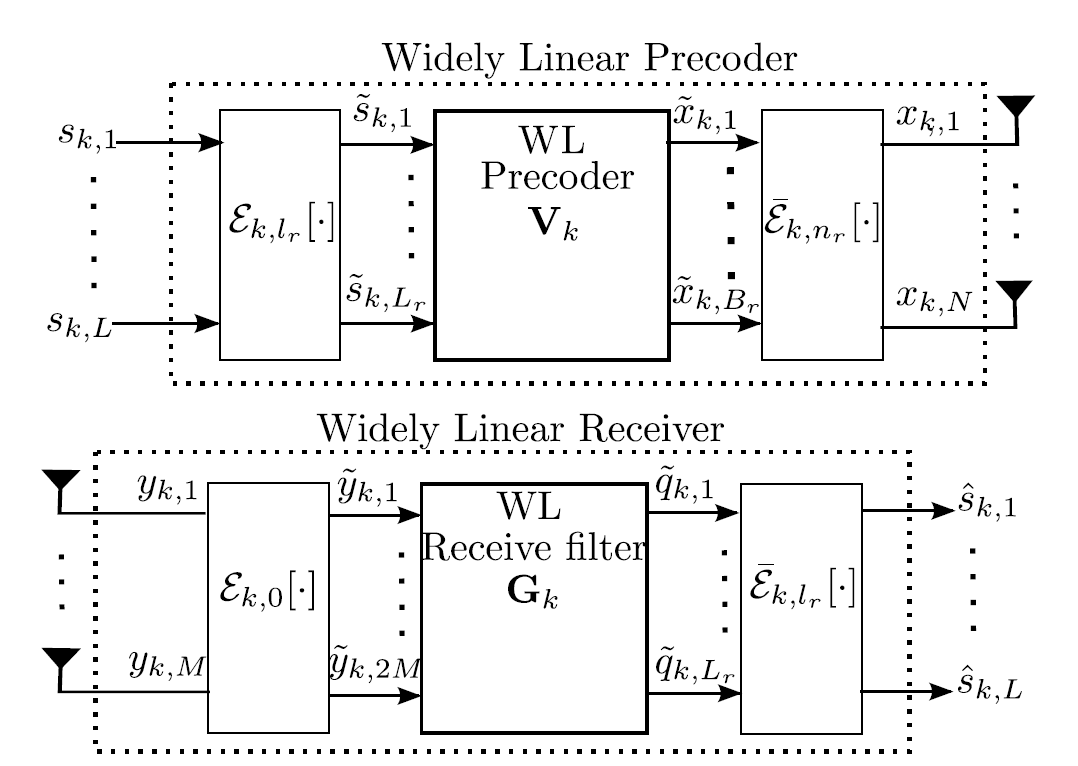
\includegraphics[width=0.7\textwidth]{figures/wl_system_model.png}
\end{center}
\caption{Block diagram of Widely Linear Transceiver} 
\label{fig:example}
\end{figure}

In this section, we discuss the system model of widely linear transceiver (WLT) for K-users MIMO channel. The system model for WLT allows one to exploit the correlation between the signals and their conjugate version. The WL processing can be performed by adopting a real-valued representation of input signals as well as the complex valued representation of input signals. We assume that input symbols of each user are drawn form the constellation which can either be real-valued or complex-valued. 

We aim to design a set of widely linear precoding and receiving filter matrices 
$((V_k,G_k), k = 1, ..., K)$
, which minimize the sum MSE under the precoding power constraints. Strictly linear filter do not exploit the correlation between signals and their conjugate version, so the strictly linear MMSE requires only the knowledge of input and noise correlation matrices $R_{s_k}$ and $R_{n_k}$ of each user, but widely linear transceiver requires the knowledge of the augmented correlation matrices
$R_{\tilde{s_k}} \hat{=} E[\tilde{s_k} \tilde{s_k^H}] $ and 
$R_{\tilde{n_k}} \hat{=} E[\tilde{n_k} \tilde{n_k^H}]$ 
of each user. In simple words, widely linear transceiver requires the knowledge of both the correlation matrix 
$R_{s_k}, R_{n_k}$ 
and the pseudo-correlation matrix 
$R_{s_k s_k^*} \hat{=} E[s_k s_k^T]$ $R_{n_k n_k^*} \hat{=} E[n_k n_k^T]$ .

The objective is to minimize the sum mean square error.

\begin{equation}
\begin{split}
	\epsilon_k =  E[ |( \, \tilde{s_k} - \tilde{z_k} ) \, ( \, \tilde{s_k} - \tilde{z_k} ) \, |^2 ] =	 \\
	((G_{k,\mu} \tilde{H}_{kk,\mu} V_{k,\mu} - I ) + \sum_{\substack{j=1 \\ j \neq k}}{G_{k,\mu}} \tilde{H}_{kj,\mu} V_{j,\mu} + G_{k,\mu} \tilde{R}_{\tilde{n}_k}) 
	\tilde{R}_{\tilde{s}} 
	((G_{k,\mu} \tilde{H}_{kk,\mu} V_{k,\mu} - I ) + \sum_{\substack{j=1 \\ j \neq k}}{G_{k,\mu}} \tilde{H}_{kj,\mu} V_{j,\mu} + G_{k,\mu} \tilde{R}_{\tilde{n}_k})^H	
\end{split}
\end{equation}

where $V_{k,\mu}$ and $ G_{k,\mu}$ are the widely linear precoder and receive filter. So, our minimization problem is formulated as follows:

\begin{equation}
	min_{\substack{V_1,...,V_K \\ G_1,...,G_K}} \sum_{k=1}^{K}{TR(\epsilon_k)}	\quad
	s.t.: Tr(V_{k,\mu}\tilde{R}_{\tilde{s}}V_{k,\mu}^H) \leq 1 \quad\quad \forall k \in {1,...,K}
\end{equation}

The optimization problem is the same as with strictly linear filter, which we will follow the same procedure. Firstly, we compute

\begin{equation}
	V_{MMSE, k}^{temp}[\mu] = ( \, \sum_{j=1}^{K}{\tilde{H}_{jk}^{H}[\mu] G_j[\mu] \tilde{R}_{\tilde{s}} G_j^H[\mu] \tilde{H}_{jk}[\mu]})^{-1} \, \tilde{H}_{kk}[\mu] G_k[\mu] \tilde{R}_{\tilde{s}}
\end{equation}

if the power constraints is fulfilled i.e, $Tr(V_{k,\mu}\tilde{R}_{\tilde{s}}V_{k,\mu}^H) \leq 1$, then $ V_{k,\mu}^{new} = V_{k,\mu}^{temp}$; otherwise, precoding is optimized according to:

\begin{equation}
	V_{MMSE, k}^{new}[\mu] = ( \, \sum_{j=1}^{K}{\tilde{H}_{jk}^{H}[\mu] G_j[\mu] \tilde{R}_{\tilde{s}} G_j^H[\mu] \tilde{H}_{jk}[\mu] + \lambda I})^{-1} \, \tilde{H}_{kk}[\mu] G_k[\mu] \tilde{R}_{\tilde{s}}
\end{equation}

where $\lambda_k $ is the Lagrange multiplier and should be $ \lambda \geq 0 $. $\lambda$ can be found by using Newton iterations with the initialization of $ \lambda = 0 $ and then update it according to:

\begin{equation}
	\lambda^{new} = \lambda^{old} + \frac{Tr( \tilde{R}_{\tilde{s}} G_k^H[\mu] \tilde{H}_{kk}[\mu] ( \, \sum_{j=1}^{K}{\tilde{H}_{jk}^{H}[\mu] G_j[\mu] \tilde{R}_{\tilde{s}} G_j^H[\mu] \tilde{H}_{jk}[\mu] + \lambda^{old} I})^{-2} \tilde{H}_{kk}^H [\mu] G_k[\mu] \tilde{R}_{\tilde{s}}) - 1}{2 \tilde{R}_{\tilde{s}} G_k^H[\mu] \tilde{H}_{kk}[\mu] ( \, \sum_{j=1}^{K}{\tilde{H}_{jk}^{H}[\mu] G_j[\mu] \tilde{R}_{\tilde{s}} G_j^H[\mu] \tilde{H}_{jk}[\mu] + \lambda^{old} I})^{-3} \tilde{H}_{kk}^H [\mu] G_k[\mu] \tilde{R}_{\tilde{s}}}
\end{equation}

until convergence is achieved or maximum number of iterations reached, where the sum MSE is decreasing with each update and therefore $v_{MMSE,k}$ reached local minimum.

The receive filter is updated according to:

\begin{equation}
	G_{MMSE, k}^{new}[\mu] = ( \, \sum_{j=1}^{K}{\tilde{H}_{kj}[\mu] V_j[\mu] \tilde{R}_{\tilde{s}} V_j^H[\mu] \tilde{H}_{kj}^H[\mu] + \sigma^2 I})^{-1} \, \tilde{H}_{kk}[\mu] V_k[\mu] \tilde{R}_{\tilde{s}}
\end{equation}


%%%%%%%%%%%%%%%%%%%%%%%%%%%%%%%%%%%%%%%%%%%%%%%%%%%%%%%%%%%%%%%%%%%%%%%%%%%%%%%

\section{Simulation results}

In this section, the simulation results are illustrated for both cases of strictly and widely linear filter using SC-FDMA modulation scheme. These are the system parameters values that defined in this system:
\begin{itemize}
	\item $M = 300, N = 512, \nu_o = 60, N_t = 2, N_r = 2$
	\item Channel: ITU-PA
	\item Realizations: 1000 as reference case, 500 for precoding
\end{itemize}


% Strictly linear filter

\begin{figure}
\centering
\begin{subfigure}{.5\textwidth}
  \centering
  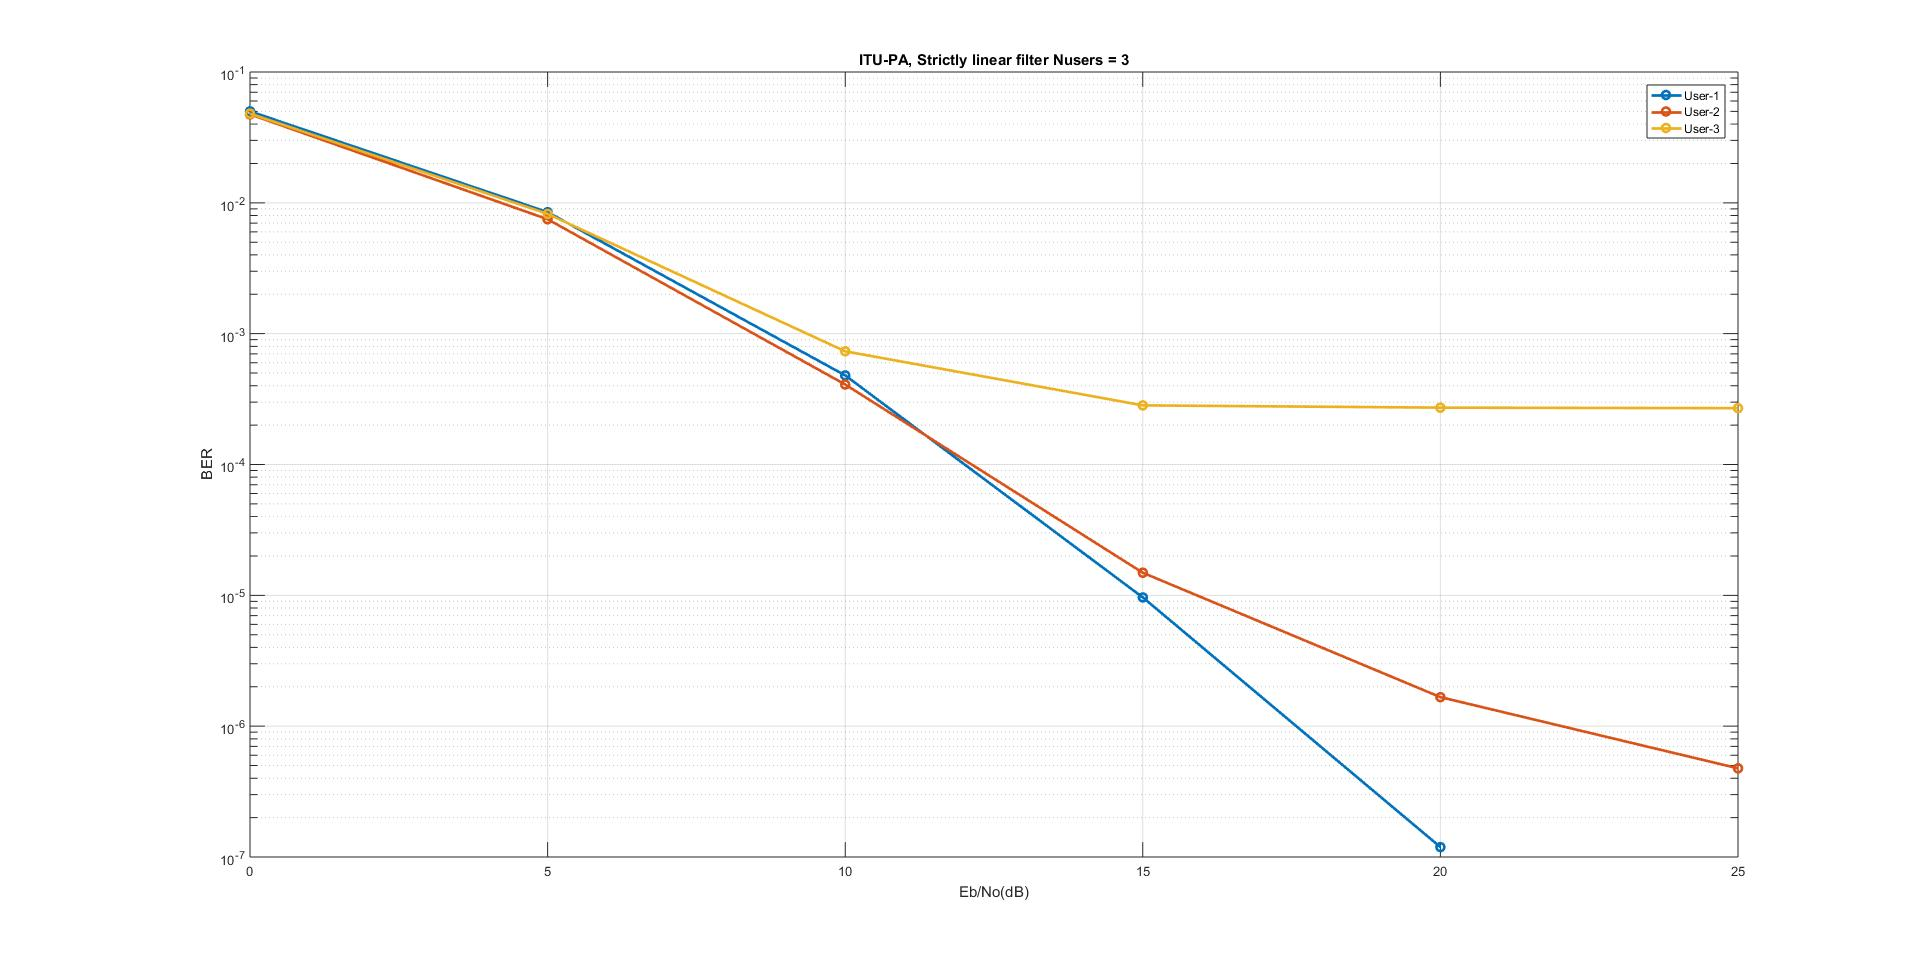
\includegraphics[width=0.9\textwidth]{figures/sl_nu3_ber}
  \caption{BER vs $E_b/N_o$} 
  \label{fig:example}
\end{subfigure}%
\begin{subfigure}{.5\textwidth}
  \centering
  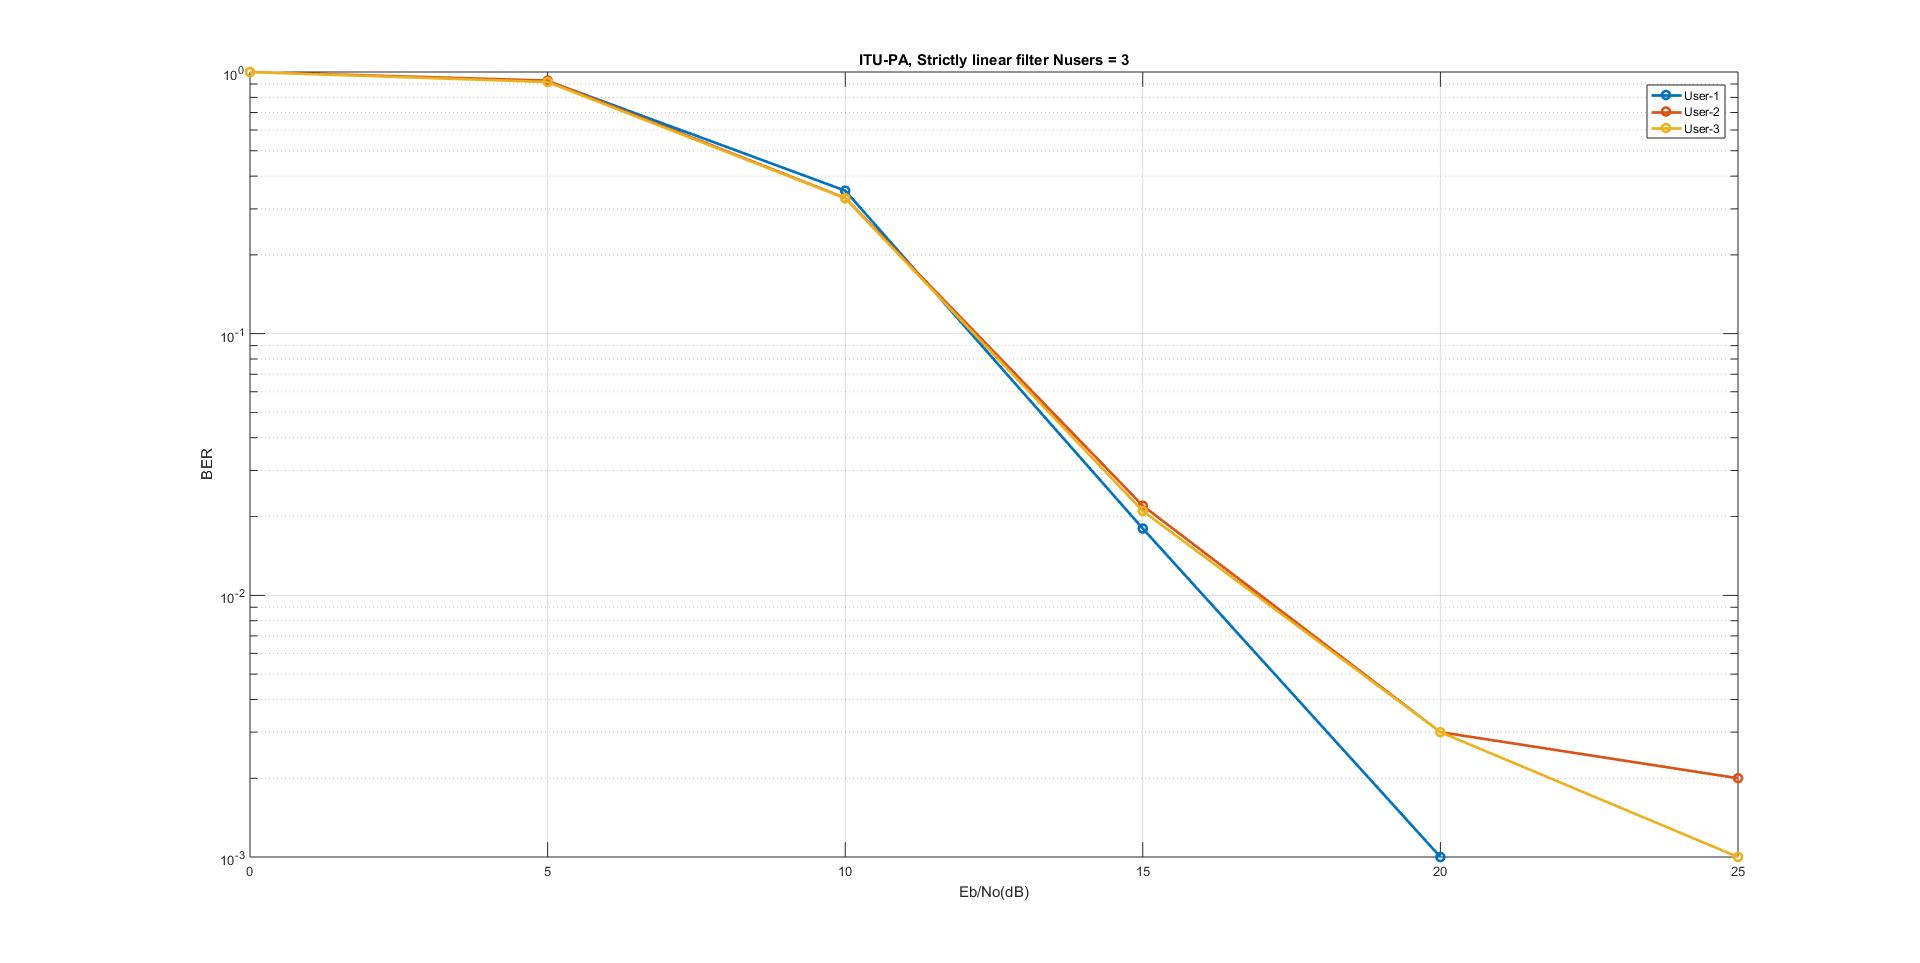
\includegraphics[width=0.9\textwidth]{figures/sl_nu3_bler}
  \caption{BLER vs $E_b/N_o$}
  \label{fig:example}
\end{subfigure}
\caption{QPSK, Strictly linear filter, $N_{users} = 3$, $N_t = N_r = 2$}
\label{fig:test}
\end{figure}

\begin{figure}
\centering
\begin{subfigure}{.5\textwidth}
  \centering
  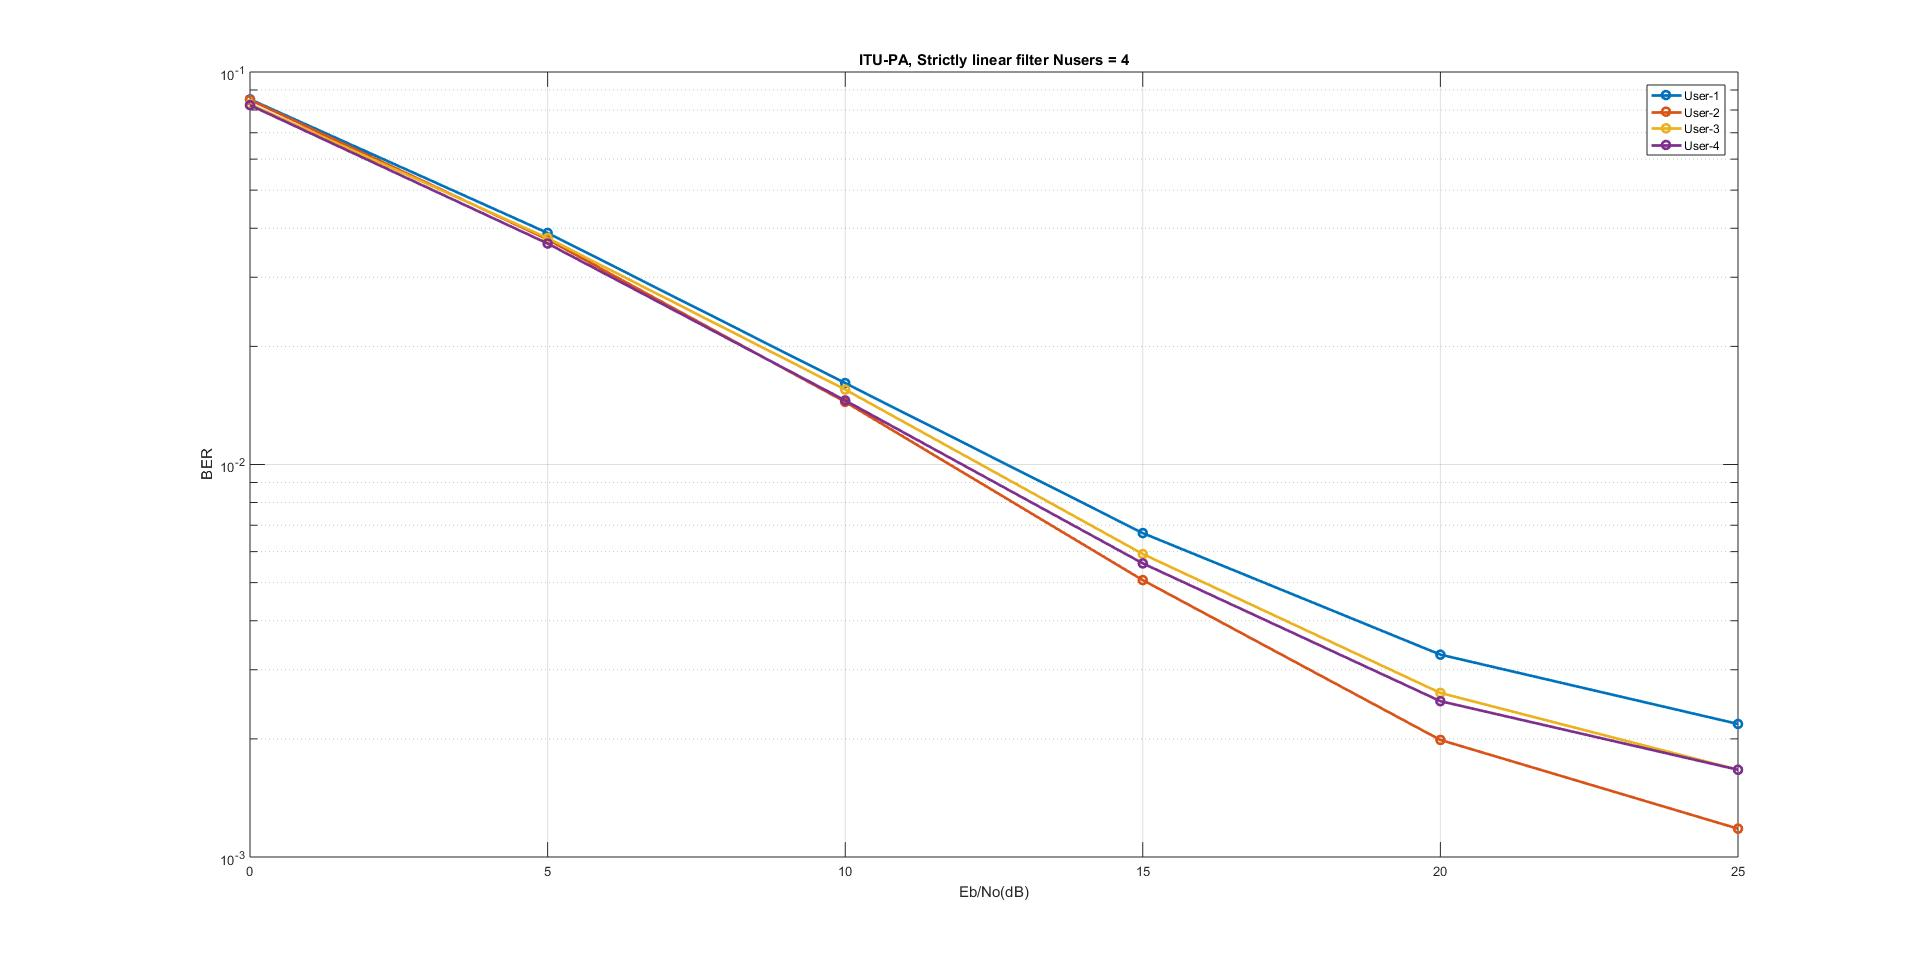
\includegraphics[width=0.9\textwidth]{figures/sl_nu4_ber}
  \caption{BER vs $E_b/N_o$} 
  \label{fig:example}
\end{subfigure}%
\begin{subfigure}{.5\textwidth}
  \centering
  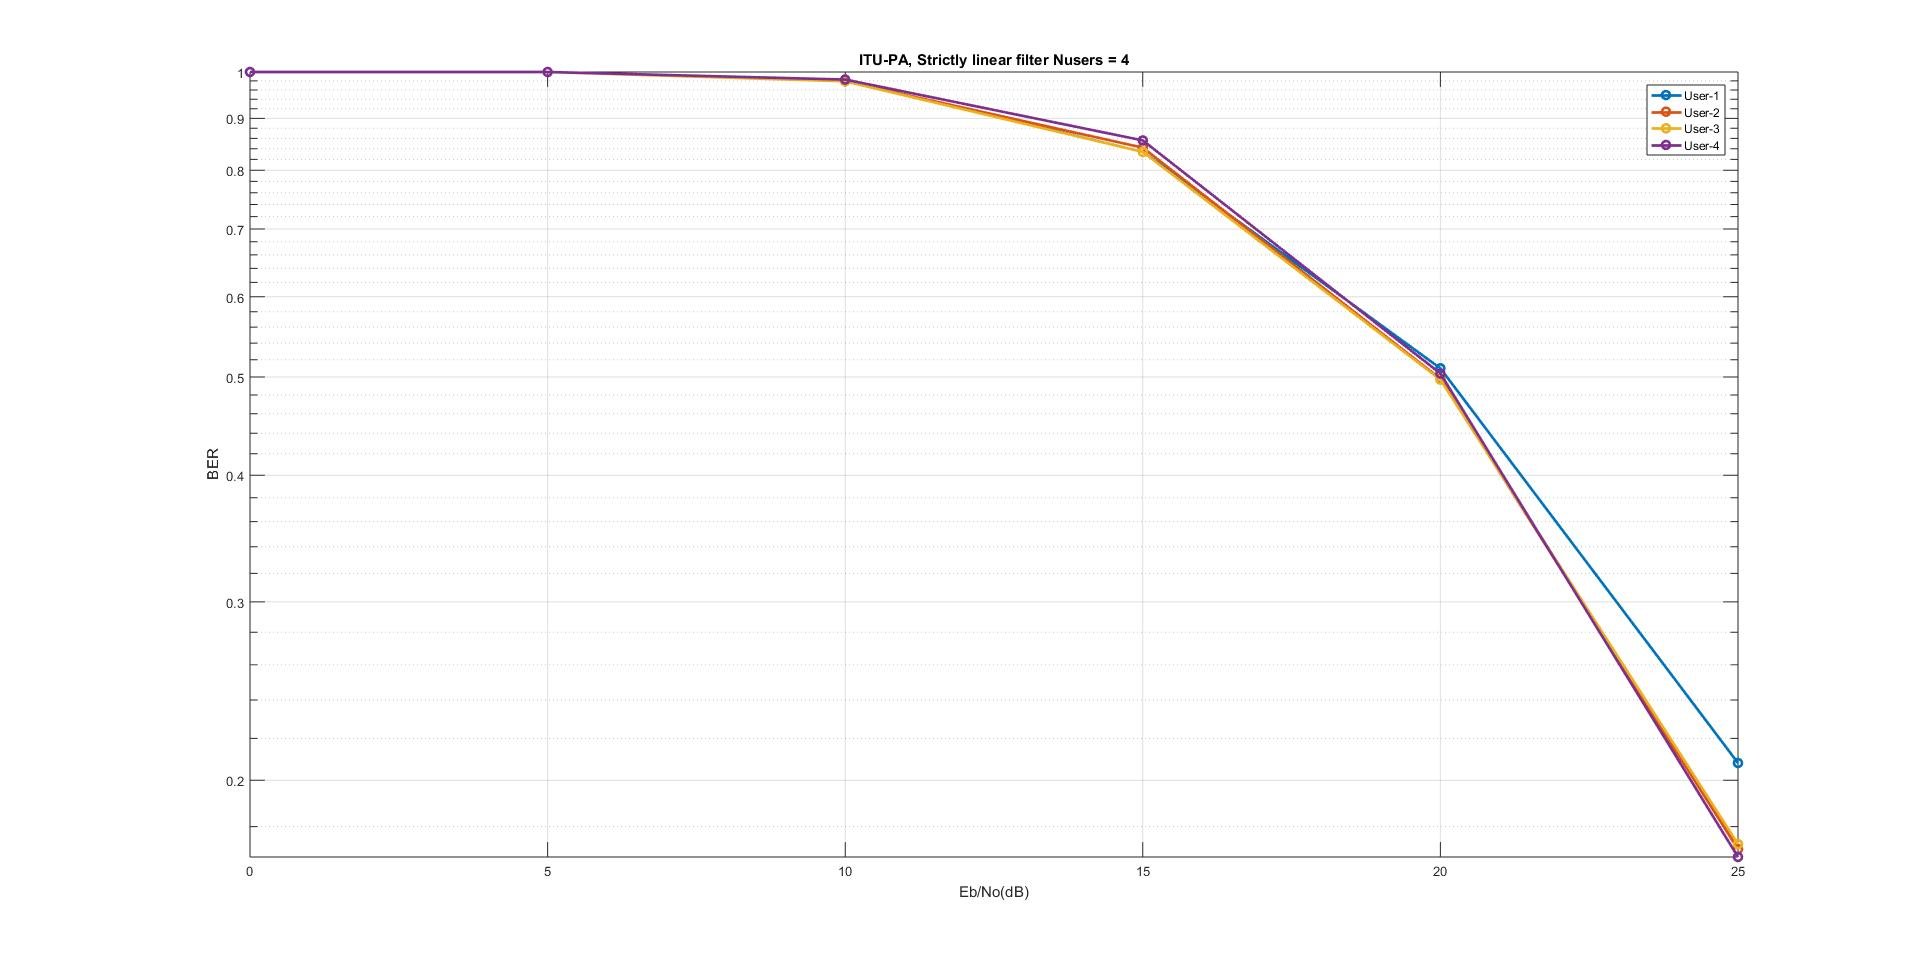
\includegraphics[width=0.9\textwidth]{figures/sl_nu4_bler}
  \caption{BLER vs $E_b/N_o$}
  \label{fig:example}
\end{subfigure}
\caption{QPSK, Strictly linear filter, $N_{users} = 4$, $N_t = N_r = 2$}
\label{fig:test}
\end{figure}


\begin{figure}
\centering
\begin{subfigure}{.5\textwidth}
  \centering
  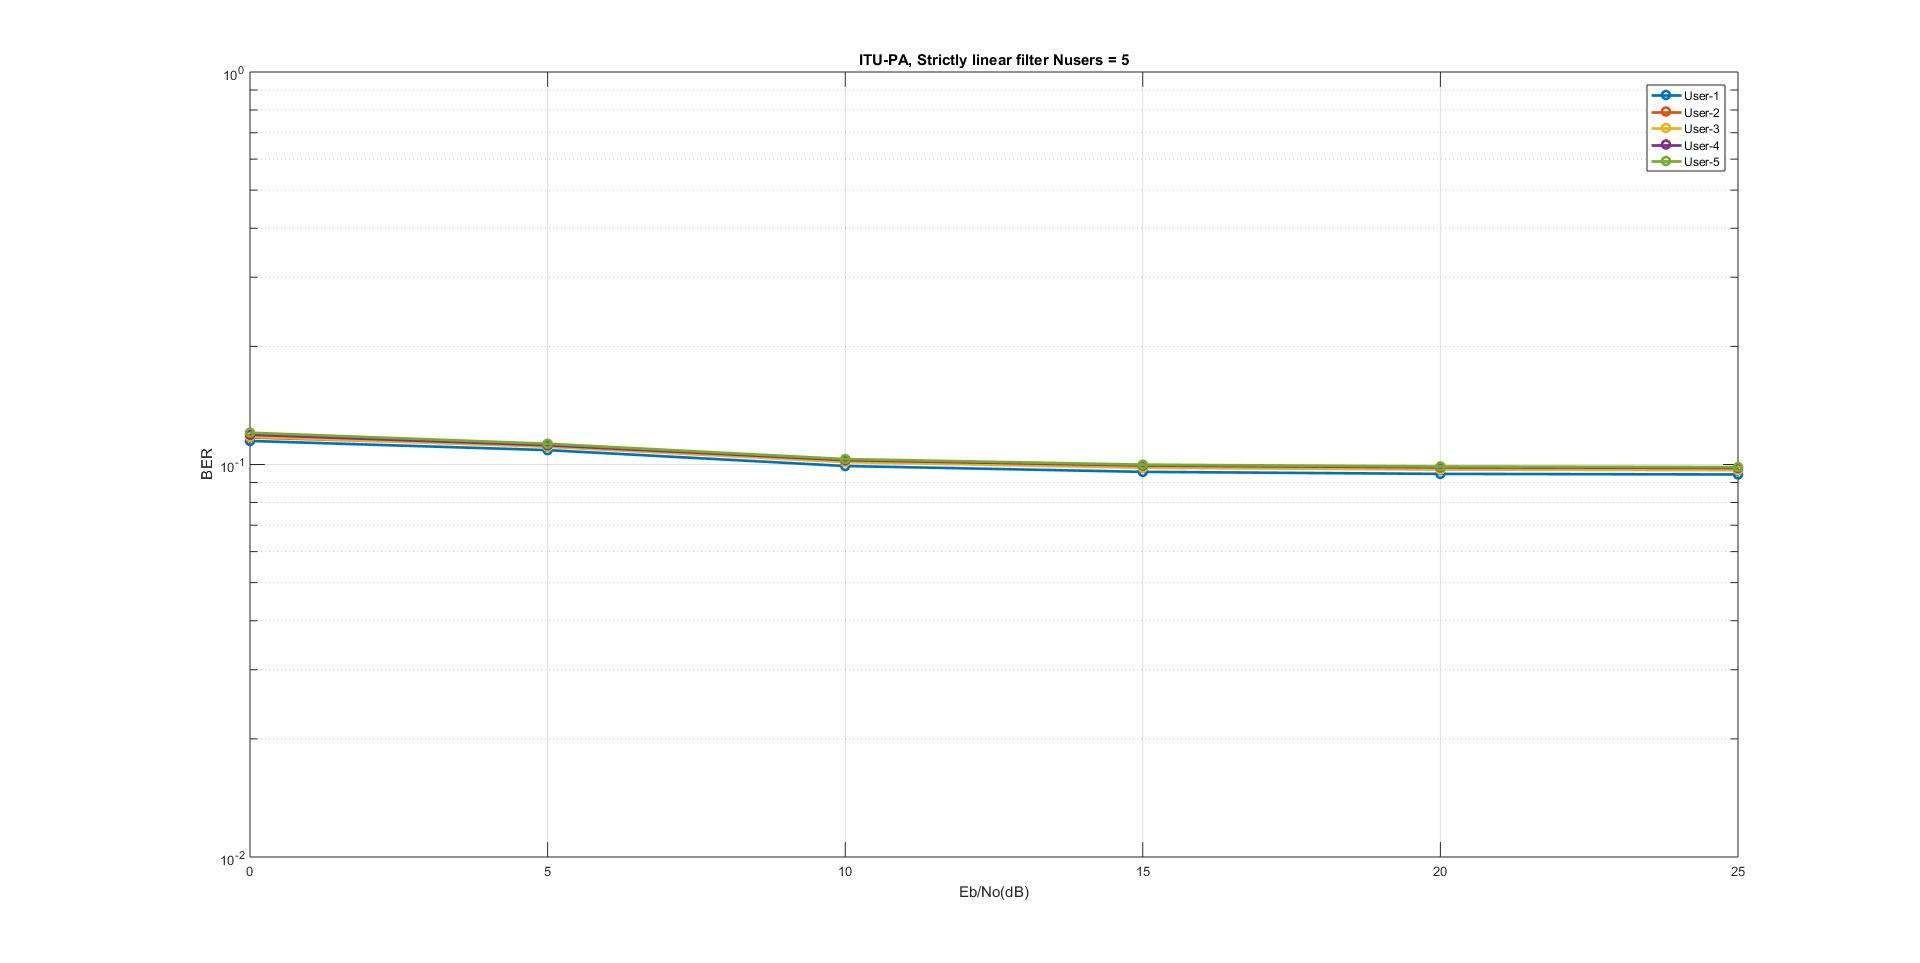
\includegraphics[width=0.9\textwidth]{figures/sl_nu5_ber}
  \caption{BER vs $E_b/N_o$} 
  \label{fig:example}
\end{subfigure}%
\begin{subfigure}{.5\textwidth}
  \centering
  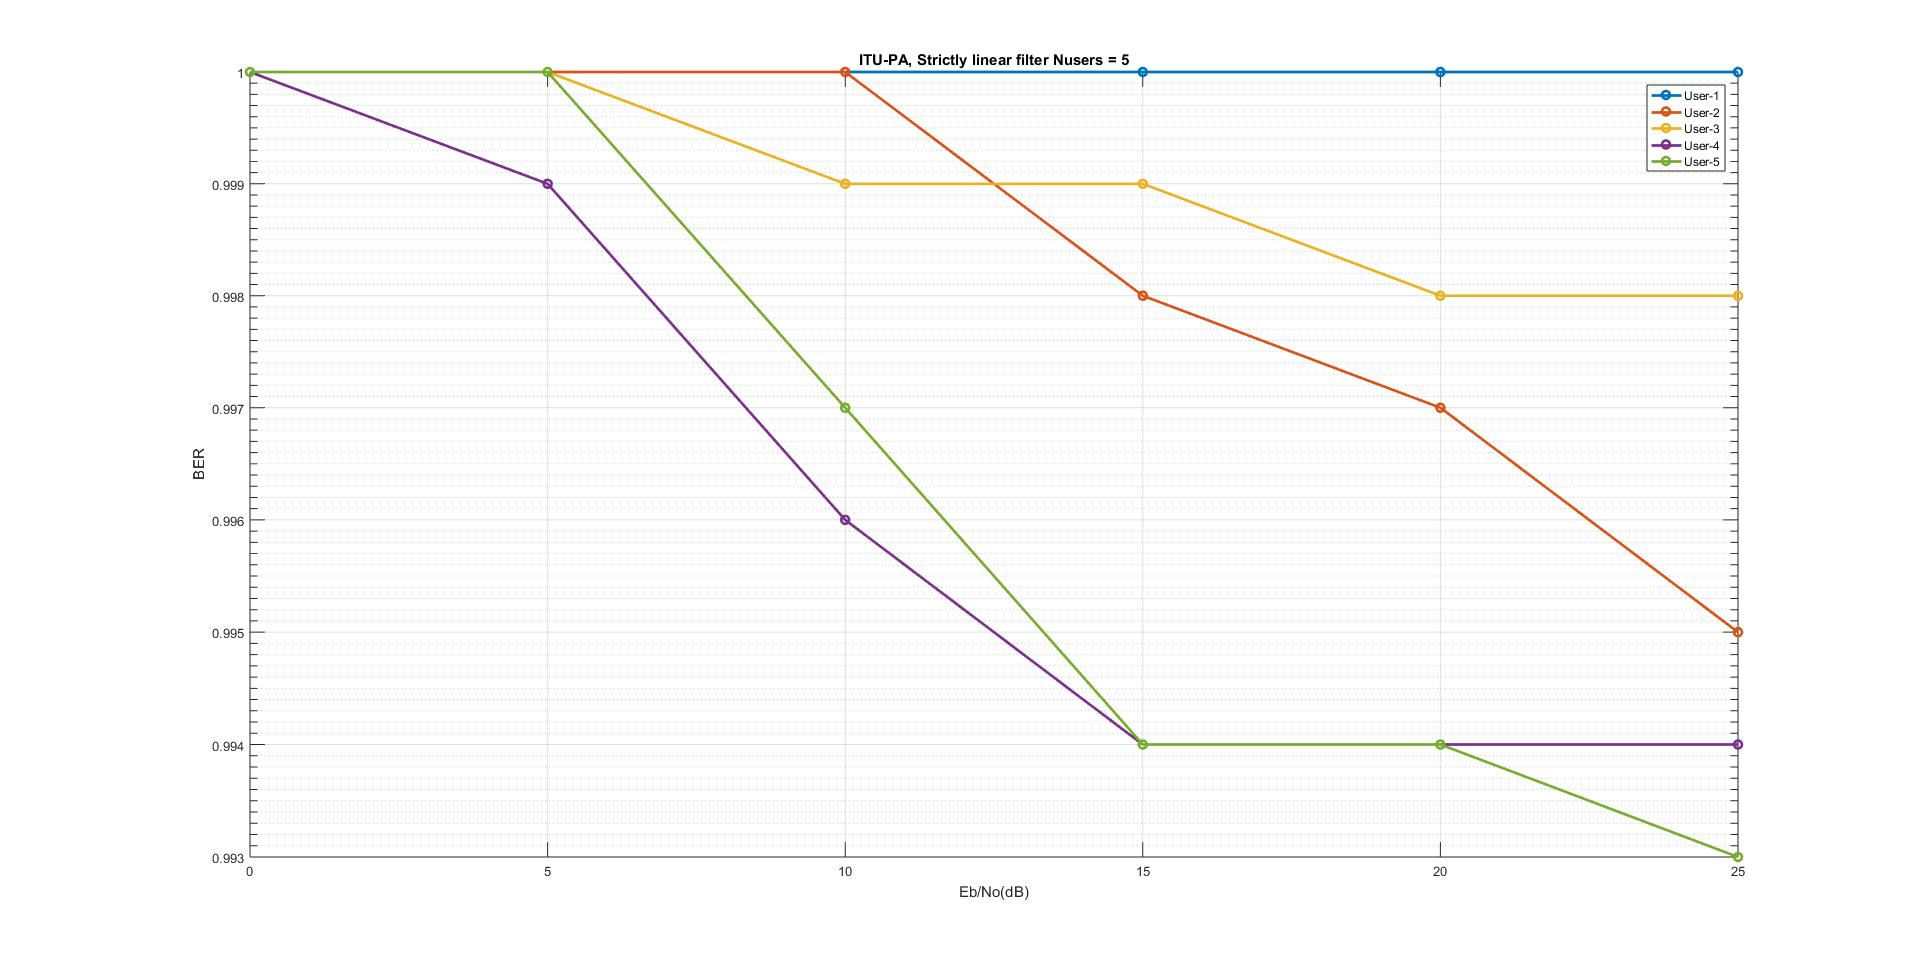
\includegraphics[width=0.9\textwidth]{figures/sl_nu5_bler}
  \caption{BLER vs $E_b/N_o$}
  \label{fig:example}
\end{subfigure}
\caption{QPSK, Strictly linear filter, $N_{users} = 5$, $N_t = N_r = 2$}
\label{fig:test}
\end{figure}

% Widely linear filter

\begin{figure}
\centering
\begin{subfigure}{.5\textwidth}
  \centering
  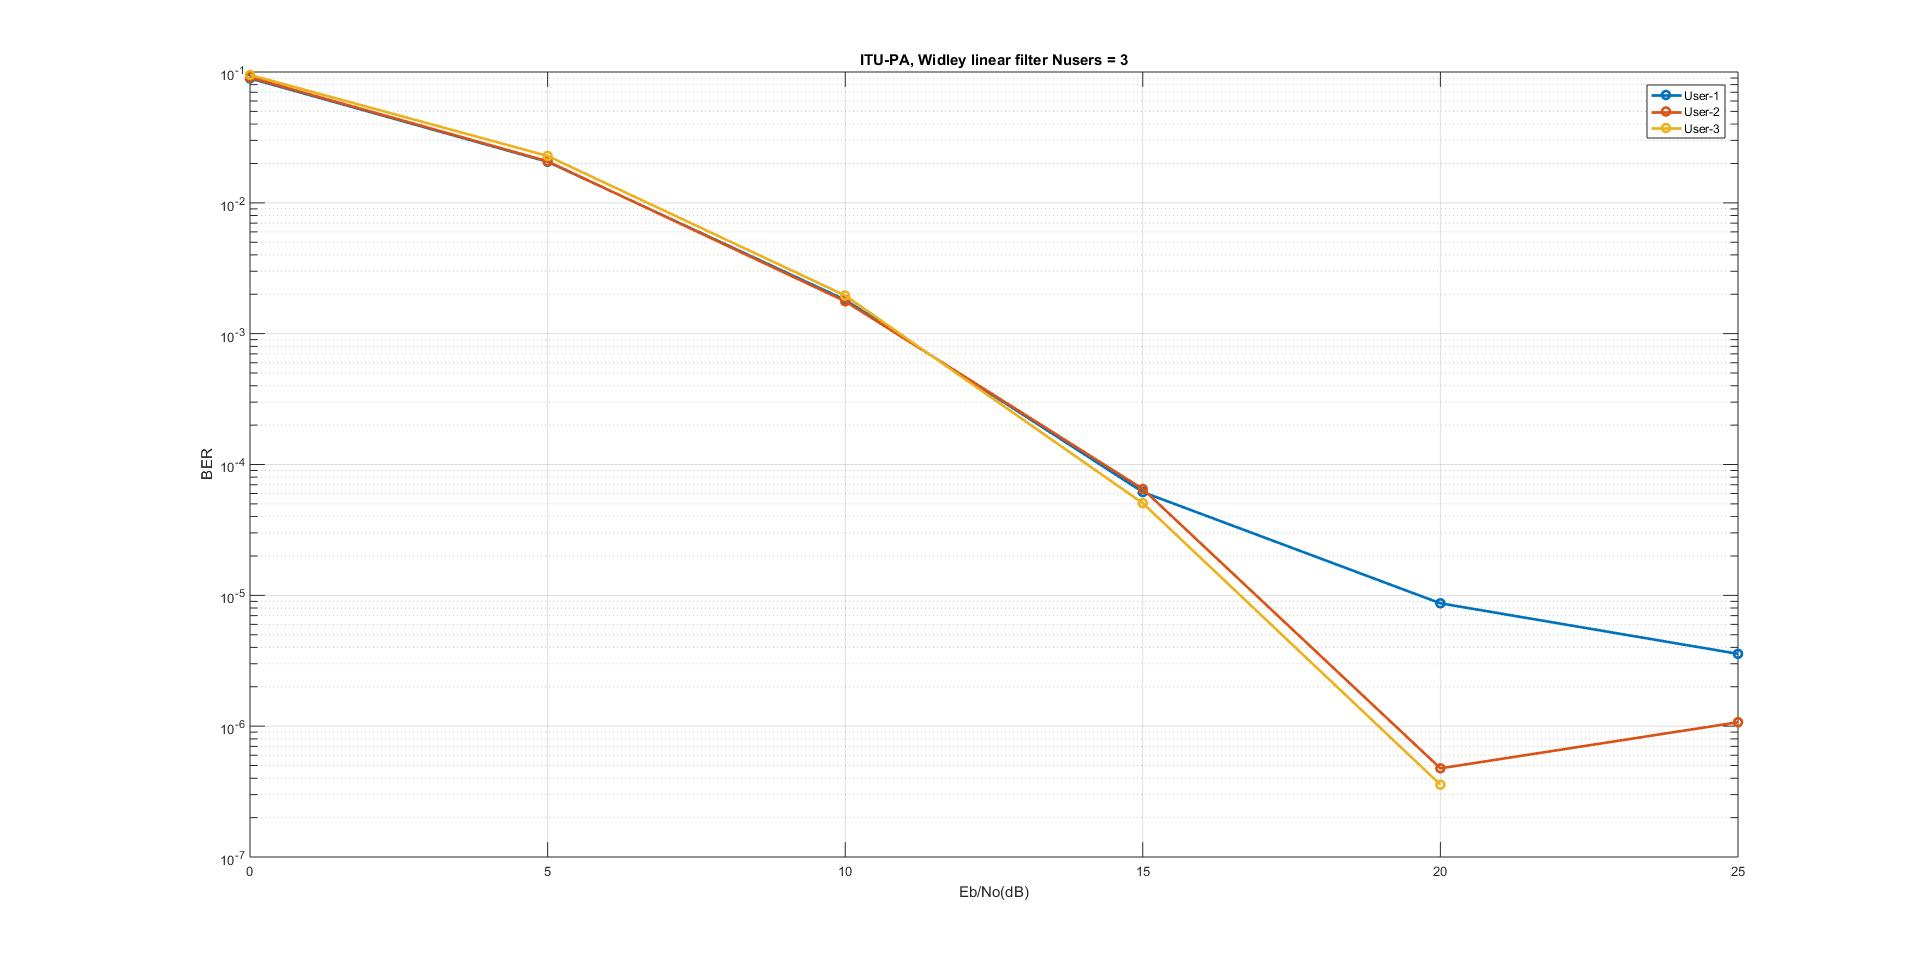
\includegraphics[width=0.9\textwidth]{figures/Wl_nu3_ber}
  \caption{BER vs $E_b/N_o$} 
  \label{fig:example}
\end{subfigure}%
\begin{subfigure}{.5\textwidth}
  \centering
  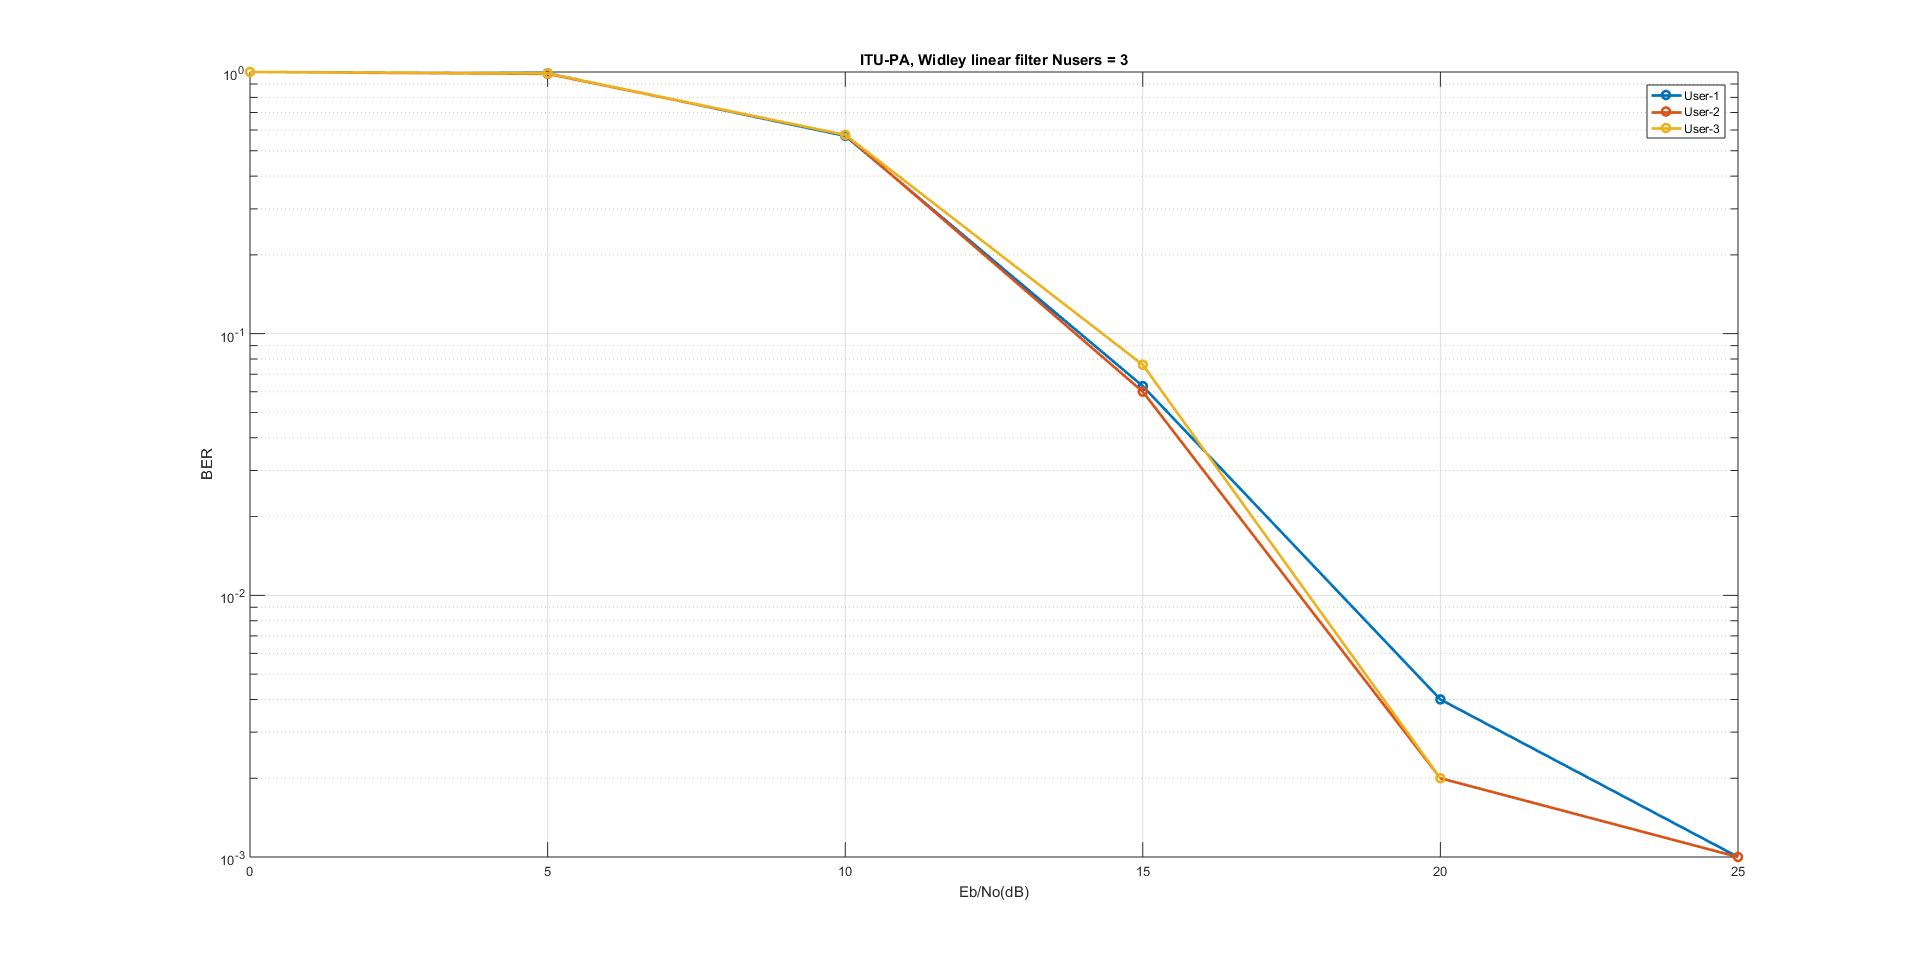
\includegraphics[width=0.9\textwidth]{figures/Wl_nu3_bler}
  \caption{BLER vs $E_b/N_o$}
  \label{fig:example}
\end{subfigure}
\caption{QPSK, Widely linear filter, $N_{users} = 3$, $N_t = N_r = 2$}
\label{fig:test}
\end{figure}


%%%%%%%%%%%%%%%%%%%%%%%%%%%%%%%%%%%%%%%%%%%%%%%%%%%%%%%%%%%%%%%%%%%%%%%%%%%%%%%
\begin{thebibliography}{Kop96}
\bibitem[1]{fb1}
Myung, Hyung G. "Introduction to single carrier FDMA." Signal Processing Conference, 2007 15th European. IEEE, 2007.


\bibitem[2]{fb2}
Schmidt, David A., et al. "Minimum mean squared error interference alignment." Signals, Systems and Computers, 2009 Conference Record of the Forty-Third Asilomar Conference on. IEEE, 2009.

\bibitem[3]{fb3} 
Dang, Uyen Ly, et al. "MMSE beamforming for SC-FDMA transmission over MIMO ISI channels with linear equalization." Global Telecommunications Conference (GLOBECOM 2010), 2010 IEEE. IEEE, 2010.	

\bibitem[4]{fb4}
Schmidt, David A., et al. "Comparison of distributed beamforming algorithms for MIMO interference networks." IEEE Transactions on Signal Processing 61.13 (2013): 3476-3489.

\bibitem[5]{fb5}
Sterle, Fabio. "Widely linear MMSE transceivers for MIMO channels." IEEE Transactions on Signal Processing 55.8 (2007): 4258-4270.



\end{thebibliography}



%%%%%%%%%%%%%%%%%%%%%%%%%%%%%%%%%%%%%%%%%%%%%%%%%%%%%%%%%%%%%%%%%%%%%%%%%%%%%%%
\end{document}
